%% 
%% Example UCD Dissertation file
%%
%% Authors: Sarah Kreidler
%%          Peter DeWitt
%%
%% Change Log: 
%% 4/13/2014 - expounded on comments and added additional figures and tables to
%%             extend the lists of figures and tables.  Added the lipsum package
%%             to this example to suppply additional meaningless text in the
%%             document.
%%             added usepackage{ctable}
%%
%% 4/13/2014 - last update by SK
%%
%% Note, this file was originall generated from the LyX editor, so some commands
%% may not be needed.  Additonal edits done in vim by PD.
%%
\documentclass[english]{ucdenver-dissertation}
\usepackage[T1]{fontenc}
\usepackage[latin9]{inputenc}
\usepackage{array}
\usepackage{float}
\usepackage{amsmath}
\usepackage{graphicx}
\usepackage{setspace}
\usepackage[authoryear]{natbib}
\doublespacing

\usepackage{ctable}

\usepackage[english]{babel}
\usepackage{blindtext}
\usepackage{lipsum}

\makeatletter

%%%%%%%%%%%%%%%%%%%%%%%%%%%%%% LyX specific LaTeX commands.  %%%%%%%%%%%%%%%%%%%
%% Special footnote code from the package 'stblftnt.sty'
%% Author: Robin Fairbairns -- Last revised Dec 13 1996
\let\SF@@footnote\footnote
\def\footnote{\ifx\protect\@typeset@protect
    \expandafter\SF@@footnote
  \else
    \expandafter\SF@gobble@opt
  \fi
}
\expandafter\def\csname SF@gobble@opt \endcsname{\@ifnextchar[%]
  \SF@gobble@twobracket
  \@gobble
}
\edef\SF@gobble@opt{\noexpand\protect
  \expandafter\noexpand\csname SF@gobble@opt \endcsname}
\def\SF@gobble@twobracket[#1]#2{}
%% Because html converters don't know tabularnewline
\providecommand{\tabularnewline}{\\}


%%%%%%%%%%%%%%%%%%%%%%%%%%%%%% User specified LaTeX commands.  %%%%%%%%%%%%%%%%%
%%\newtheorem{thm}{Theorem}
%%\newtheorem{lem}[thm]{Lemma}
%%\newdefinition{rmk}{Remark}
%%\newproof{pf}{Proof}
%%\usepackage{array}
%%\usepackage{ragged2e}
%%\newcolumntype{P}[1]{>{\RaggedLeft\hspace{0pt}}p{#1}}

%%% FRONT MATTER %%%%%%%%%%%%%%%%%%%%%%%%%%%%%%%%%%%%%%%%%%%%%%%%%%%%%%%%%%%%%%%

\title{My Kick-ass Dissertation}
\authorLast{Student}
\authorFirst{Awesome}
\authorMiddle{Q.}
\education{
B.S., Best University Ever, 2001 \\
M.S., Super Cool University, 2005
}
\school{Colorado School of Public Health}
\program{Biostatistics}
\date{2014}
\submitDate{Date-Fran-Approves-Thesis}
\advisor{Bob Q. Advisor}
\advisorTitle{Associate Professor}
\committeeChair{Susie T. Chair}
\committeeMembers{
Larry O. Committee \\
Curly O. Committee \\
Moe O. Committee
}


%% acknowledgement - this is optional
\acknowledgements{I would like to thank the academy for\ldots

  \lipsum[3]
}

%% dedication - this is also optional
\dedication{To quokkas, for being the happiest rodent on earth.}

%% sucks this has to be in here, but it's the only way I 
%% could get the latex to work
\preface{
My dissertation is about stuff.  This is the abstract describing that stuff.
Please give me a Ph.D. already. \blindtext
}

\usepackage{array}
\renewcommand\arraystretch{0.5}

\makeatother

\usepackage{babel}

%%% Begin Document %%%%%%%%%%%%%%%%%%%%%%%%%%%%%%%%%%%%%%%%%%%%%%%%%%%%%%%%%%%%%
\begin{document}

\chapter{INTRODUCTION}

Here is the mind-blowing introduction to my dissertation.  It is so awesome, you
had better sit down.  Here's some stuff another dude did \citep{article_2007}.

\lipsum

\chapter{INCREDIBLY GREAT PAPER 1%
\footnote{This chapter has been submitted for publication to the Journal of
Something Really Important by Coauthor 1 and Coauthor 2.%
}}


\section{Summary}

So you are not allowed to display an abstract in UCD formatting rules.
If you still want your abstract for each separate paper, you can add a summary
section, like this. \blindtext

\section{Introduction}

Intro stuff. \lipsum[2]

\section{Notation}

Notation section, because everyone loves math. \lipsum[3]

\section{New Methods}

Because every Ph.D. wants to make something new and fancy.

\lipsum


\section{Simulation experiment}

Because we love made up data.

\Blindtext


\section{Discussion}

Some interpretations that we totally pulled out of our, well you get the point.

\Blindtext

\newpage

\chapter{MY SECOND PAPER%
\footnote{This chapter has been submitted for publication to the Journal of Perpretual Rejection
by Coauthor 1, Coauthor2, and Coauthor 3.%
}\label{chap:paper2}}


\section{Summary}

Abstract of paper 2 \blindtext


\section{Introduction}

Wow, look at all the cool stuff I did.  You should really hire me.

\lipsum[2]


\section{Notation}

More cool math. 

\blindlist{itemize}

For $X_1, \ldots, X_n$ independent and identically distributed
from a distribution with finite mean $\mu$ and finite variance $\sigma^2,$ as $n
\rightarrow \infty$ \[ \sqrt{n} \left( \bar{X}_n - \mu \right)
\stackrel{\mathcal{L}}{\rightarrow} \mathcal{N} \left(0, \sigma^2 \right).\]

Of course you'll need to reference equation~\eqref{eq:one} too.

\begin{equation}
  1 = \int\limits_{-\infty}^{\infty} \phi \left(x \right) \mathrm{d}x 
  \label{eq:one}
\end{equation}


\section{Simulation study}

Fake data are my favorite kind of data.

\begin{figure}
\begin{centering}
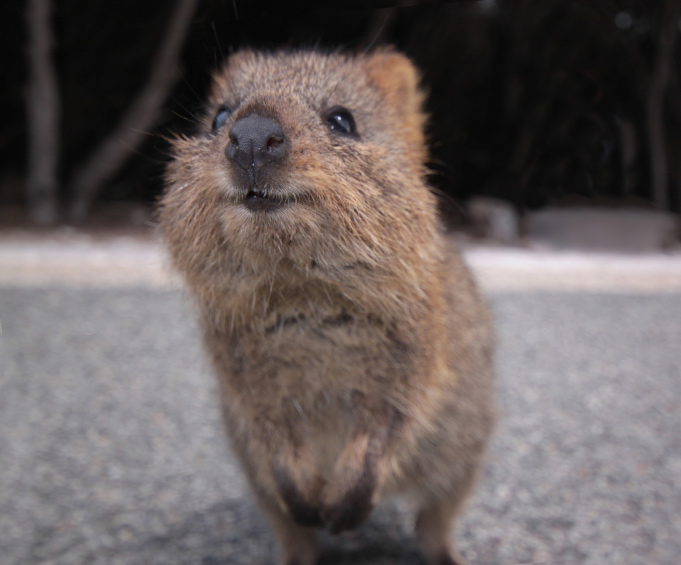
\includegraphics[width=5in]{quokka.jpg}
\par\end{centering}

\caption{Behold! The happy quokka.  Also, notice that Figure captions go below the figure}
\end{figure}

And now, a table.

\begin{table}[H]
\caption{Why quokkas are happier than you (table captions go above the table)}
\begin{centering}
\begin{tabular}{ccc}
\hline 
 & Writing a dissertation?\tabularnewline
\hline 
Quokkas & No\tabularnewline
You & Yes\tabularnewline
\hline 
\end{tabular}
\par\end{centering}

\end{table}

\section{Conclusions}

Seriously, I really need a job and look at all the stuff I just wrote!

\newpage

\chapter{MY THIRD PAPER%
\footnote{This chapter has been submitted for publication to Journal of We Secretly Love Listening 
to Abba, by Coauthor 1, Coauthor 2, Coauthor 3, and Coauthor 4.%
}}


\section{Summary}

Abstract for Paper 3 goes here. 

\blindtext


\section{Introduction}

Paper 3 will melt your eyeballs with intellectual glory.

\lipsum


\section{Notation}

I am just going to assume that every dissertation should include math,
because I am a statistician and you should be one too when you grow up.

\blindlist{itemize}



\section{New Methods}

Here is cool new math that I made up after a caffeine crazed evening
with a multivariate theory book.

\ctable[caption={Counts and row percentages for those who died by the primary
predictor, BMI, in three formats, and the secondary predictor variables as well.
Logistic regression results are presented for estimating the odds of death.
Note that there is a short caption used in the list of tables}, cap={Short
caption title for a table build with ctable},
label=tab:analysis-died,pos=H,]{lcrrrr}{}{\FL
\multicolumn{1}{l}{\bfseries }&\multicolumn{1}{c}{\bfseries }&\multicolumn{4}{c}{\bfseries Logistic Regression, Odds of Death}\NN
\cline{2-6}
\multicolumn{1}{l}{}&\multicolumn{1}{c}{}&\multicolumn{1}{c}{OR}&\multicolumn{1}{c}{lcl}&\multicolumn{1}{c}{ucl}&\multicolumn{1}{c}{p-value}\ML
{\bfseries BMI}           &  &           &      &       & \NN
~~Normal Weight           &  & Reference &      &       & \NN
~~Underweight             &  & 1.10      & 0.37 & 3.23  & 0.8656\NN
~~Overweight              &  & 1.28      & 0.69 & 2.40  & 0.4352\NN
~~Obesity Class I         &  & 1.72      & 0.86 & 3.42  & 0.1217\NN
~~Obesity Class II        &  & 1.62      & 0.69 & 3.85  & 0.2703\NN
~~Obesity Class III       &  & 2.81      & 1.10 & 7.17  & 0.0302\ML
{\bfseries Diabetes}      &  &           &      &       & \NN
~~No                      &  & Reference &      &       & \NN
~~Yes                     &  & 0.80      & 0.25 & 2.62  & 0.7131\ML
{\bfseries Pre-eclampsia} &  &           &      &       & \NN
~~No                      &  & Reference &      &       & \NN
~~Yes                     &  & 2.21      & 0.27 & 17.93 & 0.4580\ML
{\bfseries Steroids}      &  &           &      &       & \NN
~~No                      &  & Reference &      &       & \NN
~~Yes                     &  & 0.74      & 0.17 & 3.17  & 0.6803\ML
}


\section{Applied example}

Here's how to use my cool methods on real data, because I got bored with 
simulations.  And they take too long to run, anyway.



\section{Discussion}

Don't say I didn't warn you about the eyeball melting thing.

\newpage

\chapter{BIG EPIC CONCLUSION CHAPTER}

OMG, wasn't my dissertation like the coolest thing ever???!!!!

Yes it is.  So is the Colorado Avalanche winning the central division see
Figure~\ref{fig:avs-central-champs}!

\Blindtext

\begin{figure}[H]
  \center
  
\includegraphics[width=0.75\textwidth]{avs-central-champs}
  \caption{With the Blues putting up a goose egg against the Wings on the last
    day of the 2013-2014 regular season, the Avs won the division before taking
  the ice for their last game of the regular season against the Ducks.}
  \label{fig:avs-central-champs}
\end{figure}

\blindtext


\renewcommand\bibname{REFERENCES}
\singlespacing

\bibliographystyle{ucdDissertation}
\bibliography{example}


\doublespacing

%% had to do some TOC shenanigans, so please use this command instead
%% of regular old \appendix
\ucdappendix

\newpage
\chapter{MIND-ALTERING APPENDIX}

No specific formatting rules for appendices, but make sure it is awesome.  Also, here's an example of the theorem environment.

\section{Theorems}

\begin{theorem}

  Some stuff is true~\citep{article_2008}.

\end{theorem} 

\begin{proof}

Because I said so. 
\end{proof}


\end{document}
